
%%%%%%%%%%%%%%%%%%%%%%%%%%%%%%%%%%%%%%%%%%%%%%%%%%%%%%%%%% 
%%%   Find a Nice Title: #Seen #Storytelling #Events   %%%
%%%%%%%%%%%%%%%%%%%%%%%%%%%%%%%%%%%%%%%%%%%%%%%%%%%%%%%%%%

\documentclass{sig-alternate}

\usepackage{url}
\usepackage{textcomp}
\usepackage{listings}
\usepackage{color}
\usepackage{multirow}

% listing styles
\lstset{numbers=left, numberstyle=\tiny,basicstyle=\ttfamily\scriptsize, tabsize=2, keywordstyle=\underbar, stringstyle=\small, backgroundcolor=\color[gray]{0.94}, framexleftmargin=2pt}
\lstdefinestyle{rdfa}{numberblanklines=true, morekeywords={}}

% Turtle box
\definecolor{olivegreen}{rgb}{0.2,0.8,0.5}
\definecolor{grey}{rgb}{0.5,0.5,0.5}
\lstdefinelanguage{ttl}{
sensitive=true,
morecomment=[l][\color{grey}]{@},
morecomment=[l][\color{olivegreen}]{\#},
morestring=[b][\color{blue}]\",
keywordstyle=\color{cyan},
morekeywords={version,owl,rdf,rdfs,xml,xsd,dbpedia,dbo,str,sso,scms,fr,ld}
}
\lstset{
        basicstyle=\ttfamily\scriptsize,
        upquote=true,
        showspaces=false,
        showstringspaces=false,
        showtabs=false,
        tabsize=2,
        frame=none,
        breaklines,
        numbers=none,
        framexleftmargin=2mm,
        xleftmargin=2mm,
}

\newcommand{\hilight}[1]{\colorbox{yellow}{#1}}
\newcommand{\todo}[1]{\colorbox{red}{#1}}

%%%%%%%%%%%%%%%%%%%%%%%%%%%%%%%
%%%  Beginning of document  %%%
%%%%%%%%%%%%%%%%%%%%%%%%%%%%%%%

\begin{document}

\title{Find a Nice Title: \#Seen \#Storytelling \#Events}

\numberofauthors{3}
\author{
\alignauthor Carlo Andrea Conte\\
	\affaddr{Mahaya Inc.}\\
    \affaddr{New York, USA}\\
    \email{carloandreaconte@icloud.com}
\alignauthor Mor Naaman\\
    \affaddr{Cornell Tech}\\
    \affaddr{New York, USA}\\
    \email{mor.naaman@cornell.edu}
\alignauthor Rapha\"el Troncy\\
	\affaddr{EURECOM}\\
	\affaddr{Biot, France}\\
	\email{raphael.troncy@eurecom.fr}	\\
}

\maketitle

%%%%%%%%%%%%%%%%%%
%%%  Abstract  %%%
%%%%%%%%%%%%%%%%%%

\begin{abstract}
% Motivation: story is being told with links which are being shared. Describe the links processing algorithms, architecture, engineering. Describe the two algorithms that extract links (based on volume, based on velocity).

Social media platforms constitute a valuable source of information regarding real-world happenings. In particular, user generated contents on mobile-oriented platforms like Twitter allow for real-time narrations thanks to the instantaneous nature of their publishing. A common trend is to publish links to more exhaustive articles, media files and other types of information sources. In this paper, we will describe a system able to listen for tweets published regarding a particular event, for which a time-range and a set of specific hashtags are known. Such system will extract, resolve and eventually filter all the links according to a velocity-based function and a volume-based function. For each selected link, relevant information will be scraped from the referenced page.

\todo{Write conclusions reached}

\end{abstract}

% A category with the (minimum) three required fields
\category{H.3.1}{Information Storage and Retrieval}{Content Analysis and Indexing}
%\terms{Algorithms,Measurement,Experimentation,Web}
\keywords{Event, Story, Content Analysis, Seen, Twitter, Hashtags, Links}

%%%%%%%%%%%%%%%%%%%%%%%%%
%%%  1. Introduction  %%%
%%%%%%%%%%%%%%%%%%%%%%%%%

\section{Introduction}
\label{sec:introduction}

% -How people talk on Twitter about events
% -Problem of noise, quantity, quality
% -Problem of real-time computation
% -Introducing paper's sections

Social media sites like Twitter, Facebook or Instagram provide a continuous stream of user-contributed messages and media. Very often, contents are not generated within the platform itself, but are referenced via hyperlinks. The nature of these pages can be various: they can include Instagram images, news articles, real-time video streams and any other type of media. Filtering these elements and aggregating them in a storyline can offer more diverse info (to be written clearer and more discursively ---> ), more complete info, offer insights that can be complementary to an alternate fruitions of an event, the list of links itself narrates the event

Problems that have to be handles not only comprehend  filtering functions but also an architecture able to process real-time events and a way to represent results potentially very diverse results (-->scraping)

Introduction to the structure of the paper, what is where.
%%%%%%%%%%%%%%%%%%%%%%%%%
%%%  2. Related Work  %%%
%%%%%%%%%%%%%%%%%%%%%%%%%

\section{Related Work}
\label{sec:related-work}

\todo{Raphael, Mor}

%%%%%%%%%%%%%%%%%%%%%%%%%
%%%  3. Architecture  %%%
%%%%%%%%%%%%%%%%%%%%%%%%%

\section{Architecture}
\label{sec:architecture}
% Story is being told with links which are being shared. We aim to compare the kind of information we expect to obtain from this method as opposed to other ways of describing a story through social data (e.g. Seen with microblogging or other related work we pulled out in the previous section). We expect a mix of media, of which a good part will be more descriptive than a simple tweet.

User
\begin{figure}[htbp]
  \centering
  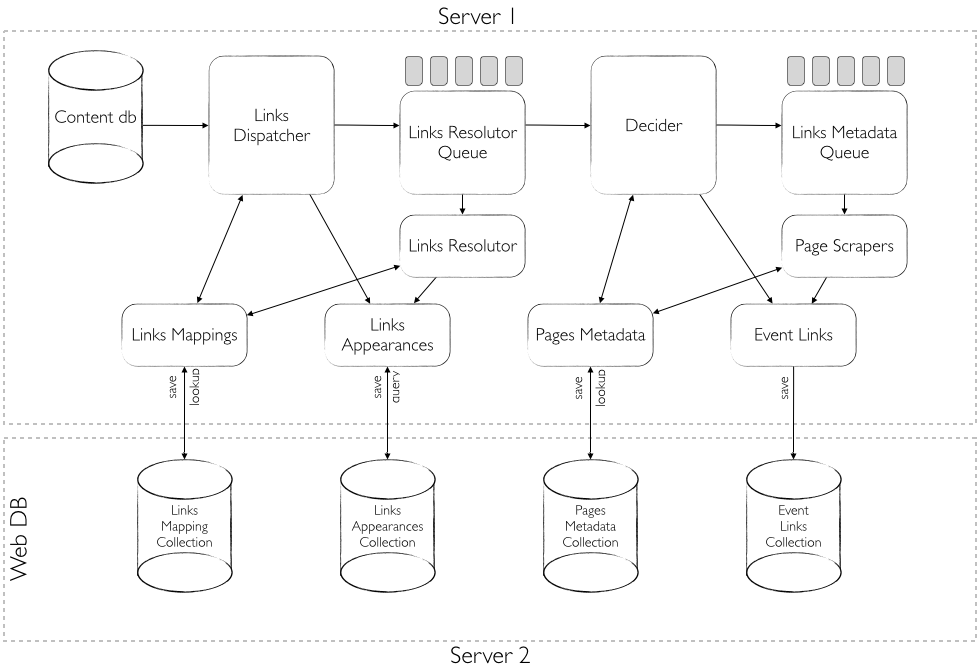
\includegraphics[width=\linewidth]{Figures/links_processing_architecture.png}
  \caption{Architecture}
  \label{fig:architecture}
\end{figure}

% Pull some statistics out of the links resolutor, with some nice charts of the SOURCES of this links OR a volume graph ordered by source, sources = registered domains.

% Compare the results for our domain of interest (news) with results from other types of event (concerts, conferences). I expect to see here something like a big slice of Instagrams, Vines, and then I hope a long tail of websites like the NYTimes or the CCN or spam bots for news events. Ideally we will be able to say how music events and tv shows have a huge amount of instant media and fewer articles, conferences have articles AND instant media, while news have a bunch of pictures of TVs tuned on the news channel and other quite redundant stuff, while the useful information resides in the long tail of domains (newspapers, blogs). 
% This requires a small addition, I just need to keep a count in the database of some information we already extract in the process, I�m sure it�s worth it.

\subsection{Volume based links selection}
LSP explanation (i.e. score function)

\subsection{Velocity based links selection}
LSP explanation

%%%%%%%%%%%%%%%%%%%%%%%%
%%%  4. Experiments  %%%
%%%%%%%%%%%%%%%%%%%%%%%%

\section{Experiments}
\label{sec:experiment}

\subsection{Dataset}
Describe what the dataset is (Seen's dataset), how data is not already organized by event, but the events database gives us the necessary info to split it.

\subsection{Volume based LSP experimental results}

Volume graphs of some approved links, explanations, interpretation of the reasons

\subsection{Velocity based LSP experimental results}

Cross validation: In the previous two subsections we can pretty much only validate the precision of the two algorithms together. How about considering the set of elements that were not selected in one algorithm, but were selected in the other one and vice versa to see if one has a better recall?

%%%%%%%%%%%%%%%%%%%%%%%%%%%%%%%%%
%%%  5. Building a Storyline  %%%
%%%%%%%%%%%%%%%%%%%%%%%%%%%%%%%%%

\section{Building a Storyline}
\label{sec:storyline}
We should place the selected links (selected based on any method we decided was better for this scope between the previous two) in chronological order and see if they actually follow the evolution of the story, with what granularity. This will only work with a long event.


%%%%%%%%%%%%%%%%%%%%%%%%%%%%%%%%%%%%%%%
%%%  6. Conclusion and Future Work  %%%
%%%%%%%%%%%%%%%%%%%%%%%%%%%%%%%%%%%%%%%

\section{Conclusion and Future Work}
\label{sec:conclusions}


\section{Acknowledgments}
\label{sec:ack}

\nocite{*}
\bibliographystyle{abbrv}
\bibliography{seen}
\balancecolumns
% That's all folks!
\end{document} 
